\begin{flushright} {\tiny {\color{gray} python\_codes/fieldstone\_134/text.tex}} \end{flushright}

%\lstinputlisting[language=bash,basicstyle=\small]{python_codes/fieldstone_01/keywords}

\begin{center}
\inpython Codes at \url{https://github.com/cedrict/fieldstone/tree/master/python_codes/fieldstone_134}
\end{center}

\par\noindent\rule{\textwidth}{0.4pt}

{\sl This stone was developed in collaboration with Neil Ribe}. \index{contributors}{N. Ribe}

\par\noindent\rule{\textwidth}{0.4pt}
%%%%%%%%%%%%%%%%%%%%%%%%%%%%%%%%%%%%%%%%%%%%%%%%%%%%%%%%%%%%%%%%%%%%%%%%%%%%%%%%%%%%%%%%%%%%%%

%taken from http://rcmt2.bo.ingv.it/
The seismic moment tensor is a complete description of the earthquake size and source geometry. 
The Centroid Moment Tensor (CMT) is a reliable method for calculating moment tensors, 
by which the Global Centroid Moment Tensor Project systematically studies global seismicity 
starting from the 80's.

Q: what is a seimic tensor? \url{https://mxrap.com/moment-tensors-a-practical-guide/}


All what follows is to be found at \url{https://www.globalcmt.org/}.
Also check \textcite{eknd12} (2012) for an overview of the project.

The available data is stored in the "ndk" file format which used to store
and distribute the Global Centroid-Moment-Tensor (CMT) catalog
(formerly the Harvard CMT catalog).
The format is ASCII and uses five 80-character lines per earthquake. 
Example\footnote{I have added the blanklines. In the file there are none.}:

\begin{center}
\begin{verbatim}
================================================================================
12345678901234567890123456789012345678901234567890123456789012345678901234567890

PDE  2005/01/01 01:20:05.4  13.78  -88.78 193.1 5.0 0.0 EL SALVADOR             
C200501010120A   B:  4    4  40 S: 27   33  50 M:  0    0   0 CMT: 1 TRIHD:  0.6
CENTROID:     -0.3 0.9  13.76 0.06  -89.08 0.09 162.8 12.5 FREE S-20050322125201
23  0.838 0.201 -0.005 0.231 -0.833 0.270  1.050 0.121 -0.369 0.161  0.044 0.240
V10   1.581 56  12  -0.537 23 140  -1.044 24 241   1.312   9 29  142 133 72   66

PDE  2005/01/01 01:42:24.9   7.29   93.92  30.0 5.1 0.0 NICOBAR ISLANDS, INDIA R
C200501010142A   B: 17   27  40 S: 41   58  50 M:  0    0   0 CMT: 1 TRIHD:  0.7
CENTROID:     -1.1 0.8   7.24 0.04   93.96 0.04  12.0  0.0 BDY  S-20050322125628
23 -1.310 0.212  2.320 0.166 -1.010 0.241  0.013 0.535 -2.570 0.668  1.780 0.151
V10   3.376 16 149   0.611 43  44  -3.987 43 254   3.681 282 48  -23  28 73 -136

....

================================================================================
\end{verbatim}
\end{center}

\begin{itemize}
\item First line: Hypocenter line\\
\verb|[1-4]|   Hypocenter reference catalog (e.g., PDE for USGS location, ISC for
               ISC catalog, SWE for surface-wave location, \textcite{ekst06} (2006))\\
\verb|[6-15]|  Date of reference event\\
\verb|[17-26]| Time of reference event\\
\verb|[28-33]| Latitude\\
\verb|[35-41]| Longitude\\
\verb|[43-47]| Depth\\
\verb|[49-55]| Reported magnitudes, usually mb and MS\\
\verb|[57-80]| Geographical location (24 characters)

\item Second line: CMT info (1)\\
\verb|[1-16]|  CMT event name. This string is a unique CMT-event identifier. Older
        events have 8-character names, current ones have 14-character names.
        See note (1) below for the naming conventions used.\\
\verb|[18-61]| Data used in the CMT inversion. Three data types may be used: 
        Long-period body waves (B), Intermediate-period surface waves (S),
        and long-period mantle waves (M). For each data type, three values
        are given: the number of stations used, the number of components 
        used, and the shortest period used.\\
\verb|[63-68]| Type of source inverted for: "CMT: 0" - general moment tensor; 
        "CMT: 1" - moment tensor with constraint of zero trace (standard); 
        "CMT: 2" - double-couple source.\\
\verb|[70-80]| Type and duration of moment-rate function assumed in the inversion. 
        "TRIHD" indicates a triangular moment-rate function, "BOXHD" indicates
        a boxcar moment-rate function. The value given is half the duration
        of the moment-rate function. This value is assumed in the inversion,
        following a standard scaling relationship (see note (2) below),
        and is not derived from the analysis.
        
\item Third line: CMT info (2)\\
\verb|[1-58]|  Centroid parameters determined in the inversion. Centroid time ({\python C\_time}), given
        with respect to the reference time, centroid latitude ({\python C\_lat}), 
        centroid longitude ({\python C\_lon}), and centroid depth ({\python C\_depth}). 
        The value of each variable is followed
        by its estimated standard error. See note (3) below for cases in
        which the hypocentral coordinates are held fixed.\\
\verb|[60-63]| Type of depth. "FREE" indicates that the depth was a result of the
        inversion; "FIX " that the depth was fixed and not inverted for;
        "BDY " that the depth was fixed based on modeling of broad-band 
        P waveforms.\\
\verb|[65-80]| Timestamp. This 16-character string identifies the type of analysis that
        led to the given CMT results and, for recent events, the date and 
        time of the analysis. This is useful to distinguish Quick CMTs ("Q-"), 
        calculated within hours of an event, from Standard CMTs ("S-"), which 
        are calculated later. The format for this string should not be 
        considered fixed.

\item Fourth line: CMT info (3)\\
\verb|[1-2]| The exponent for all following moment values. For example, if the
        exponent is given as 24, the moment values that follow, expressed in 
        dyne-cm, should be multiplied by 10**24.\\
\verb|[3-80]| The six moment-tensor elements: $M_{rr}$, $M_{tt}=M_{\theta\theta}$, 
        $M_{pp}=M_{\phi\phi}$, $M_{rt}$, $M_{rp}$, $M_{tp}$, 
        where $r$ is up, $t$ is south, and $p$ is east. See Aki and Richards book \cite{akirichards}
        for conversions to other coordinate systems. The value of each moment-tensor
        element is followed by its estimated standard error. See note (4)
        below for cases in which some elements are constrained in the inversion.
        
\item Fifth line: CMT info (4)\\
\verb|[1-3]|   Version code. This three-character string is used to track the version 
        of the program that generates the "ndk" file.\\
\verb|[4-48]|  Moment tensor expressed in its principal-axis system: eigenvalue, 
        plunge, and azimuth of the three eigenvectors. The eigenvalue should be
        multiplied by 10**(exponent) as given on line four.\\
\verb|[50-56]| Scalar moment, to be multiplied by 10**(exponent) as given on line four.\\
\verb|[58-80]| Strike, dip, and rake for first nodal plane of the best-double-couple 
        mechanism, repeated for the second nodal plane. The angles are defined
        as in Aki and Richards book \cite{akirichards}.

\end{itemize}
          
        
Notes (additional information):
\begin{enumerate}
\item CMT event names follow two conventions. Older events use an 8-character 
name with the structure XMMDDYYZ, where MMDDYY represents the date of
the event, Z is a letter (A-Z followed by a-z) distinguishing different 
events on the same day, and X is a letter (B,M,Z,C,...) used to identify 
the types of data used in the inversion. Newer events use 14-character event 
names with the structure XYYYYMMDDhhmmZ, in which the time is given to greater
precision, and the initial letter is limited to four possibilities: B - body 
waves only, S - surface waves only, M - mantle waves only, C - a combination 
of data types.

\item The source duration is generally estimated using an empirically determined
relationship such that the duration increases as the cube root of the scalar
moment. Specifically, we currently use a relationship where the half duration
for an event with moment 10**24 is 1.05 seconds, and for an event with moment
10**27 is 10.5 seconds.

\item For some small earthquakes for which the azimuthal distribution of stations 
with useful seismograms is poor, we constrain the epicenter of the event to
the reference location. This is reflected in the catalog by standard 
errors of 0.0 for both the centroid latitude and the centroid longitude.

\item For some very shallow earthquakes, the CMT inversion does not well 
constrain the vertical-dip-slip components of the moment tensor ($M_{rt}$ and $M_{rp}$),
and we constrain these components to zero in the inversion. The standard
errors for $M_{rt}$ and $M_{rp}$ are set to zero in this case.
\end{enumerate}

\vspace{1cm}

Problems I have noticed with the data file:
line 69823: 1.060.0 becomes 1060.0 ?
line 73622: 6.010.0 becomes 6010.0 ? 


\begin{center}
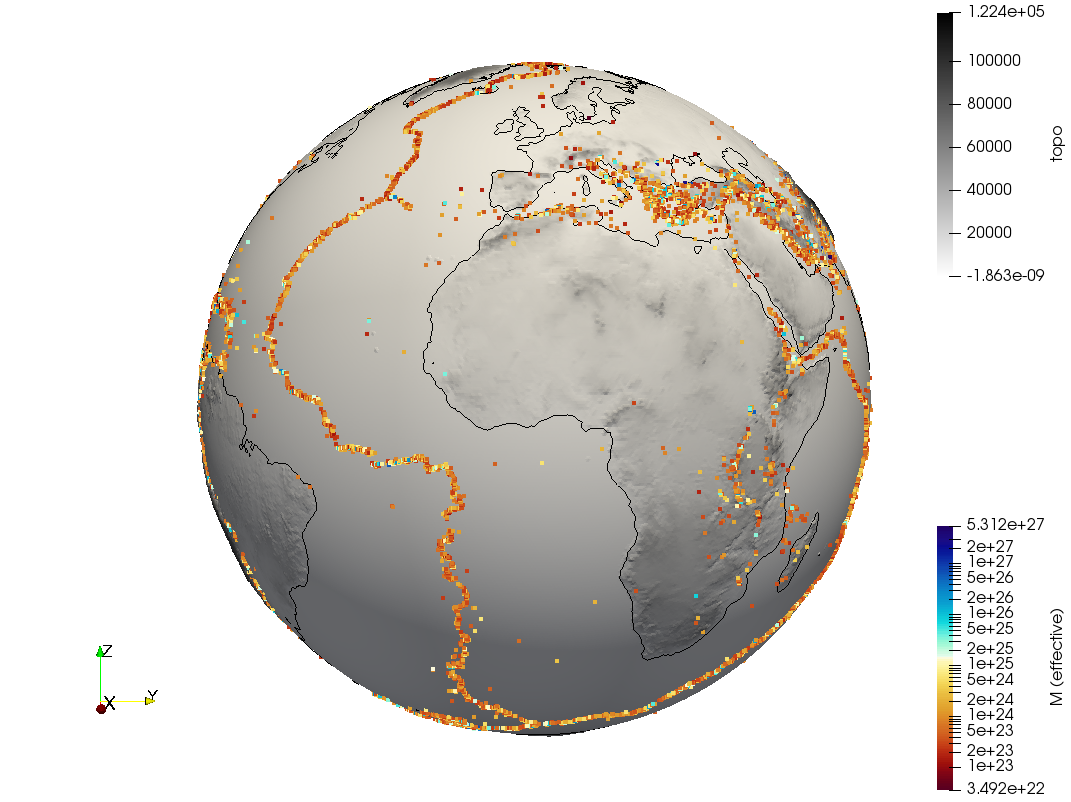
\includegraphics[width=5cm]{python_codes/fieldstone_134/images/visu1}
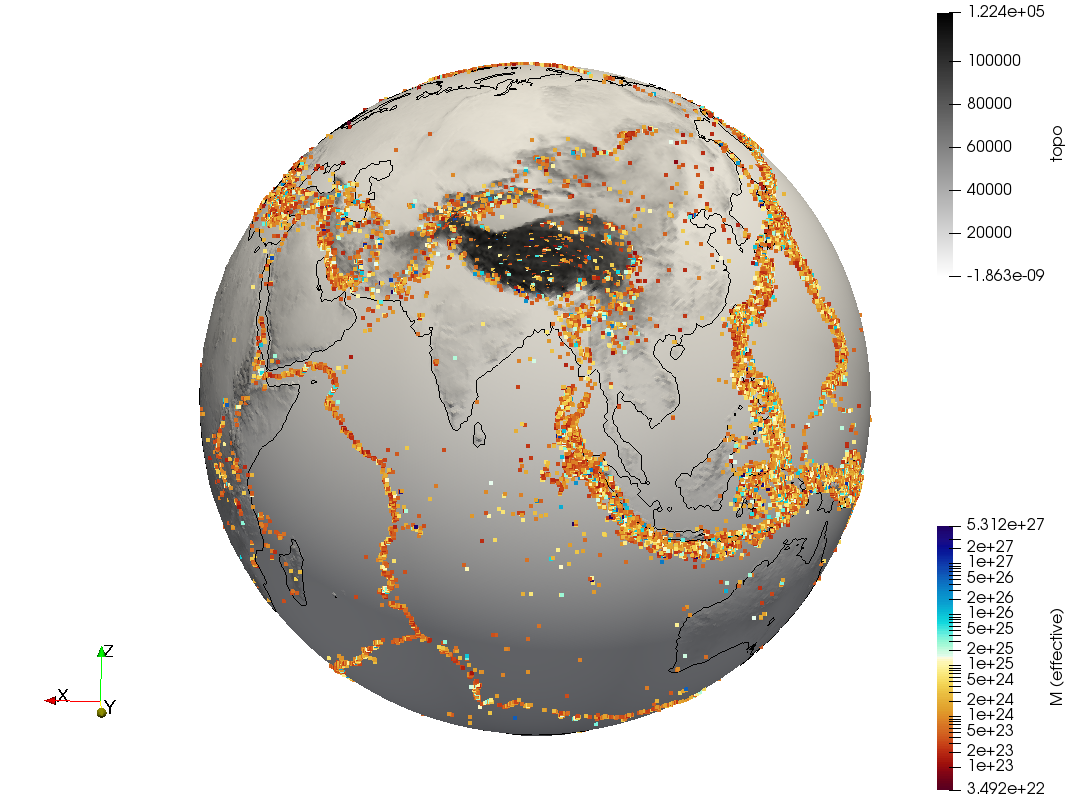
\includegraphics[width=5cm]{python_codes/fieldstone_134/images/visu2}
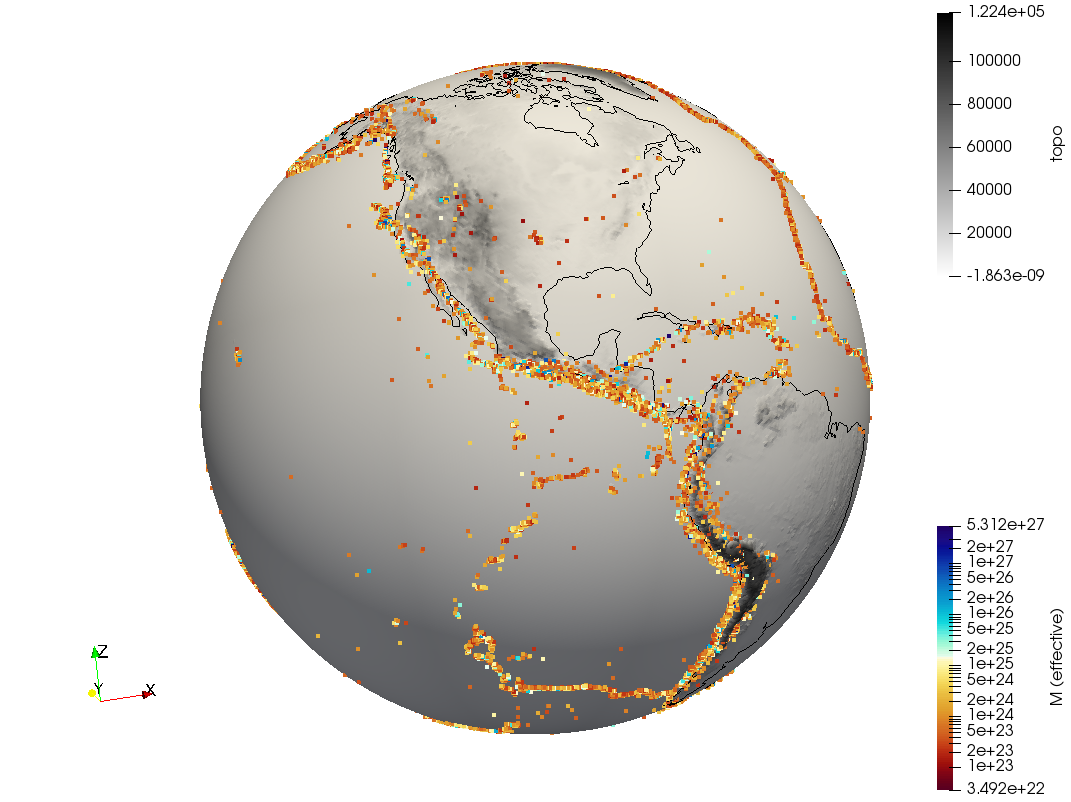
\includegraphics[width=5cm]{python_codes/fieldstone_134/images/visu3}
\end{center}

%---------------------------------------------------------------------------------- 

There seems to be another catalogue
for the European-Mediterranean Regional Centroid-Moment Tensors
at \url{http://rcmt2.bo.ingv.it/}.


\begin{center}
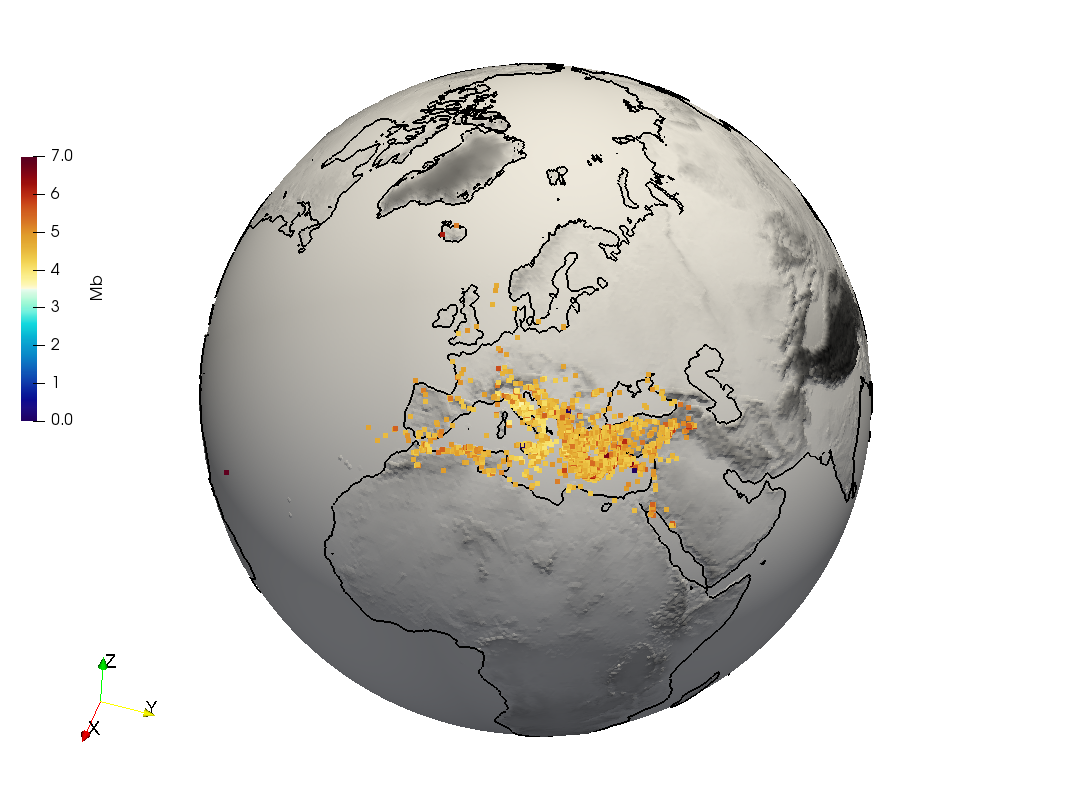
\includegraphics[width=5cm]{python_codes/fieldstone_134/images/visu5}
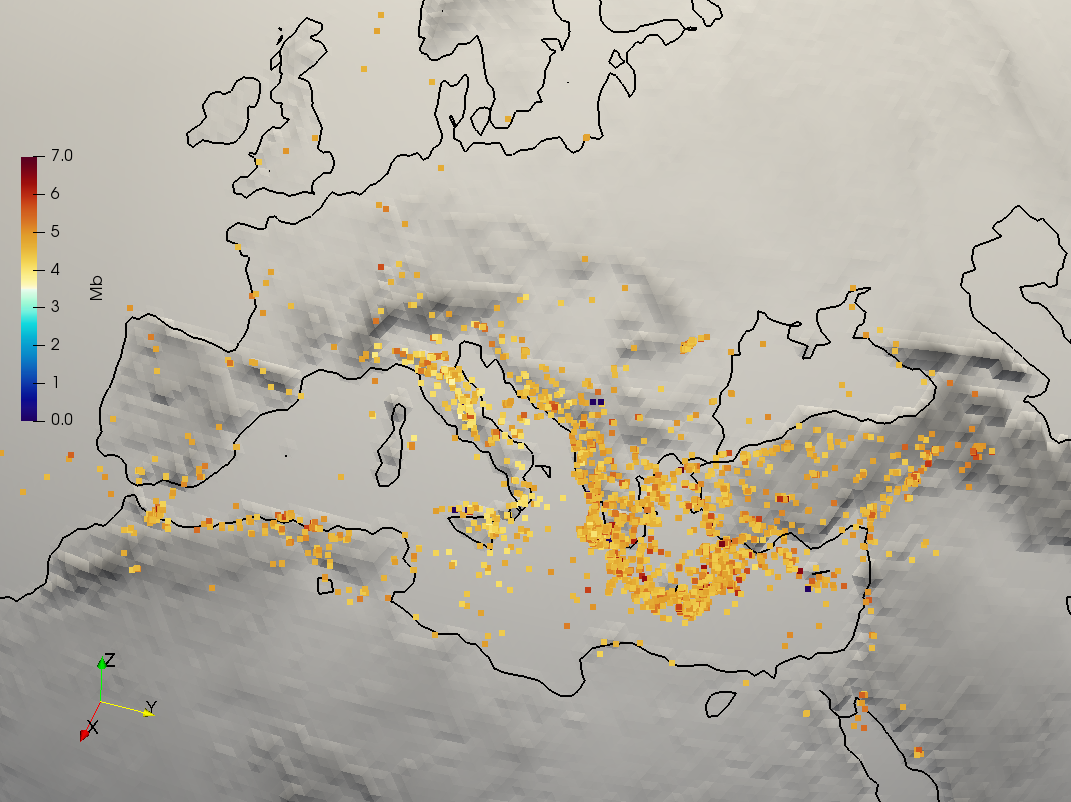
\includegraphics[width=5cm]{python_codes/fieldstone_134/images/visu4}
\end{center}


